\section{支架零件图制作}
\begin{procedure}

\begin{figure}[htbp]
\centering
\subfloat[]{\label{fig:layoutwizard1}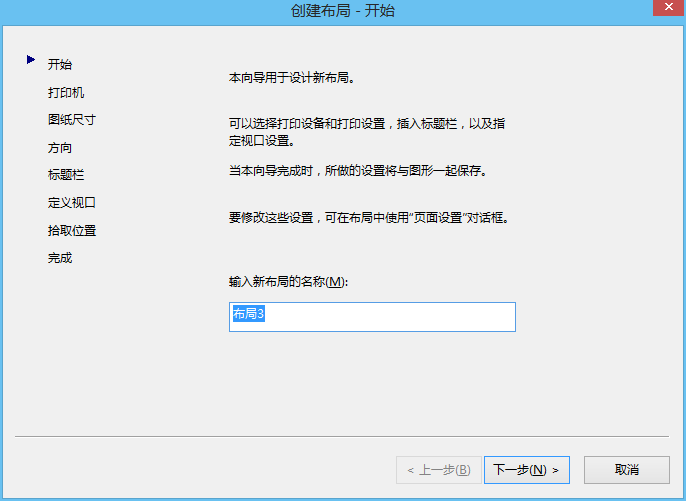
\includegraphics[scale=0.15]{layoutwizard1}}\hspace{20pt}
\subfloat[]{\label{fig:layoutwizard2}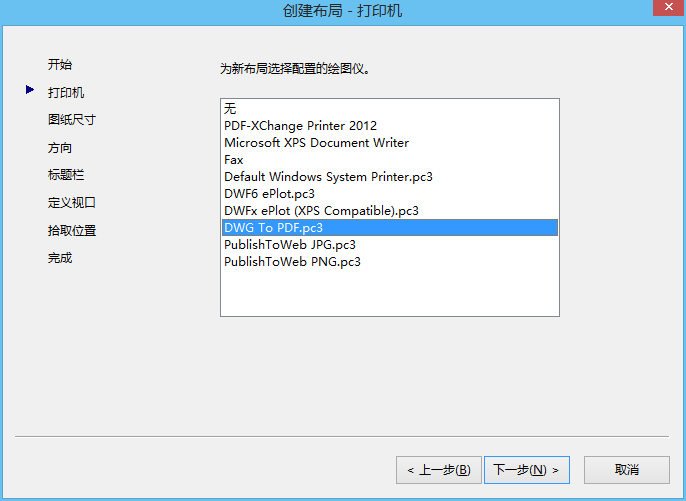
\includegraphics[scale=0.15]{layoutwizard2}}\hspace{20pt}
\subfloat[]{\label{fig:layoutwizard3}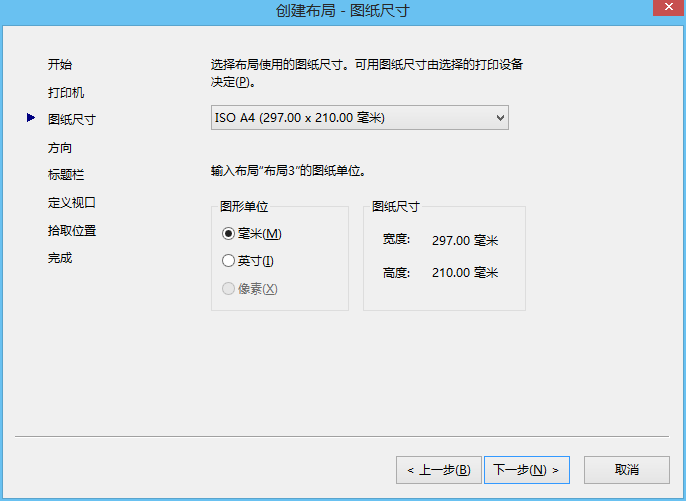
\includegraphics[scale=0.15]{layoutwizard3}}
\caption{新建布局过程(一)}
\end{figure}

\item 创建新布局

由于系统创建的窗口布局通常是不能够满足实际布局需求的,为适应支架三视图生成的需要,我们可以采用新建布局向导来进行设置。AutoCAD中调用新建布局向导的方法有:
\begin{itemize}
\item 键盘输入layoutwizard\index{layoutwizard,创建布局向导}
\item 【插入】$\rightarrow $【布局】$\rightarrow $【创建布局向导】
\end{itemize}

调用布局向导命令会弹出图\ref{fig:layoutwizard1}所示的创建布局对话框,在文本框中输入新布局的名称;点击下一步进入图\ref{fig:layoutwizard2}所示的打印机设置步骤,将打印机设置为“DWG TO PDF.pc3”;点击下一步进入图\ref{fig:layoutwizard3}所示的图纸尺寸设置步骤,将图纸尺寸设置为“ISO A4(297.00x210.00毫米)";点击下步进入图\ref{fig:layoutwizard4}所示的方向设置步骤,由于A4图纸比较小,对放置三视图而言设置为纵向比较合理,故选择纵向;点击下一下进入图\ref{fig:layoutwizard5}所示的标题栏设置步骤,由于无符合国家标准的标题栏,故选择无;点击下一步进入图\ref{fig:layoutwizard6}所示的定义视口步骤,为方便后续操作,将其设置为无视口;点击下一步进入图\ref{fig:layoutwizard7}完成布局创建。

\begin{figure}[htbp]
\centering
\subfloat[]{\label{fig:layoutwizard4}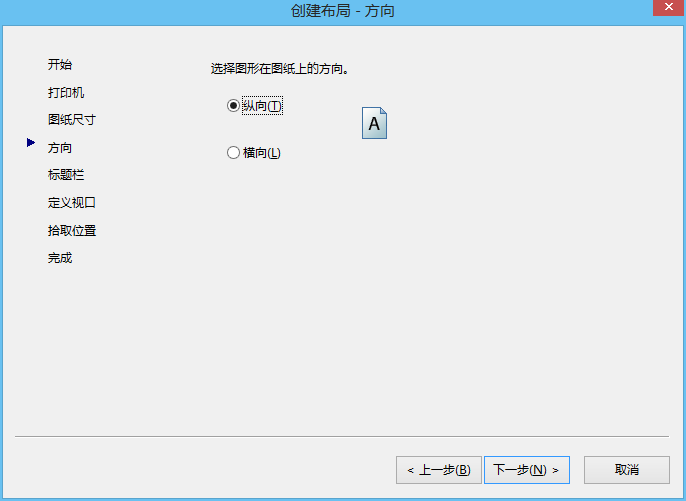
\includegraphics[scale=0.15]{layoutwizard4}}\hspace{20pt}
\subfloat[]{\label{fig:layoutwizard5}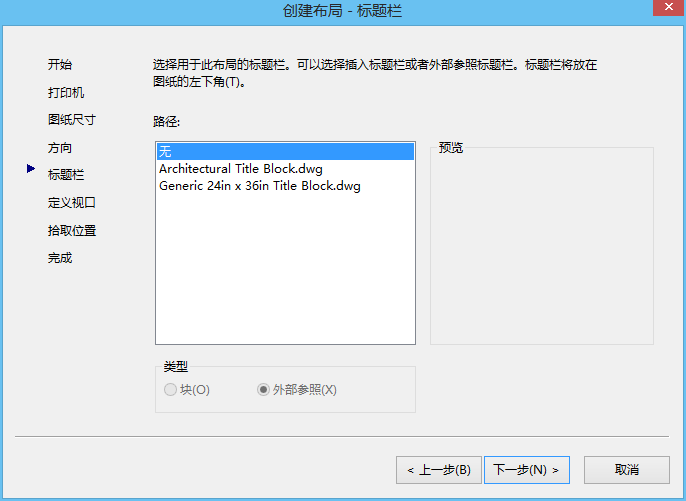
\includegraphics[scale=0.15]{layoutwizard5}}\hspace{20pt}
\subfloat[]{\label{fig:layoutwizard6}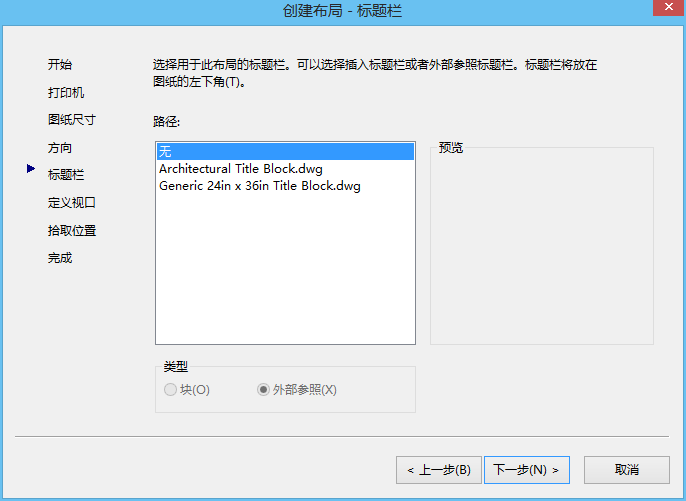
\includegraphics[scale=0.15]{layoutwizard5}}
\caption{新建布局过程(二)}
\end{figure}
\begin{lstlisting}
命令:LAYOUTWIZARD
\end{lstlisting}

\begin{figure}[htbp]
\centering
\subfloat[]{\label{fig:layoutwizard7}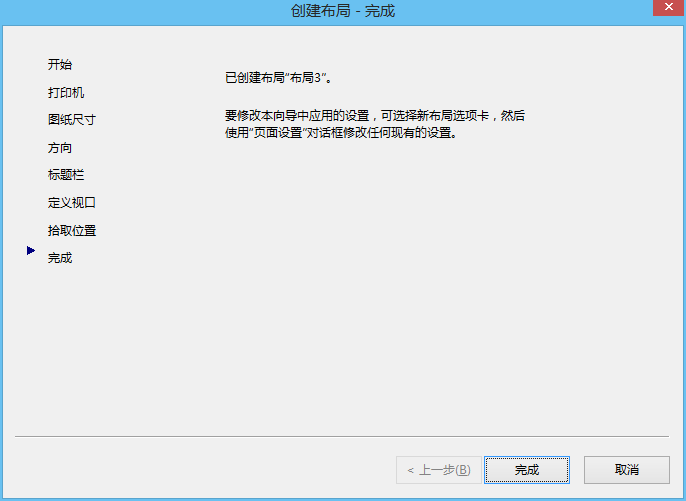
\includegraphics[scale=0.25]{layoutwizard7}}\hspace{20pt}
\subfloat[]{\label{fig:zhijiabuju1}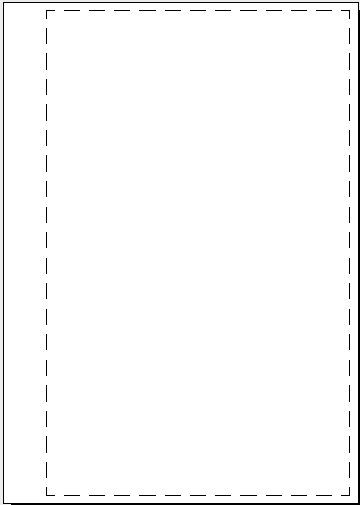
\includegraphics[scale=0.3]{zhijiabuju1}}
\caption{新建布局过程(三)}
\end{figure}

通过向导创建的布局其可打印区域通常不能够与标准图幅的要求是不一致的,因此需要利用页面设置管理器设置图纸可打印区域,最终结果如图\ref{fig:zhijiabuju1}所示。

\item 新建图层

新建“尺寸标注”和“标题栏”图层,线型为“continuous",线宽为默认;新建“中心线”图层,线型为“center",线宽为默认; 新建“图框”图层,线型为“continuous",线宽为0.5mm。

\item 制作图框与标题栏

设置当前图层为“图框”,绘制图框矩形。
\begin{lstlisting}
命令: RECTANG
指定第一个角点或 [倒角(C)/标高(E)/圆角(F)/厚度(T)/宽度(W)]: 0,0
指定另一个角点或 [面积(A)/尺寸(D)/旋转(R)]: @180,287
\end{lstlisting}

设置当前图层为“标题栏”,插入“GB标题栏”块。
\begin{lstlisting}
命令: INSERT
指定插入点或 [基点(B)/比例(S)/旋转(R)]:
\end{lstlisting}

\begin{figure}[htbp]
\centering

\end{figure}
\item 加载虚线线型

为方便于生成视图时系统自动设置虚线,需要先加载虚线线型。在AutoCAD中加载线型可调用线型管理器,其调用方式为:
\begin{itemize}
\item 键盘输入linetype\index{linetype}
\item 【格式】$\rightarrow $【线型】
\end{itemize}

调用线型管理器命令会弹出图\ref{fig:linetypemanarge}所示的对话框,点击加载按钮,并加载“HIDDEN”线型,结果如图\ref{fig:loadhiddenline}所示。

\begin{figure}[htbp]
\centering
\subfloat[]{\label{fig:linetypemanarge}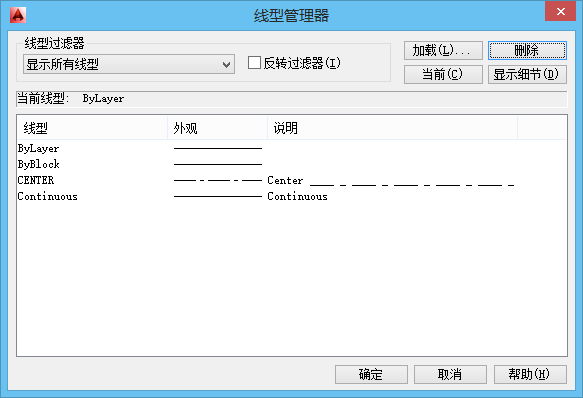
\includegraphics[scale=0.35]{linetypemanarge}}\hspace{20pt}
\subfloat[]{\label{fig:loadhiddenline}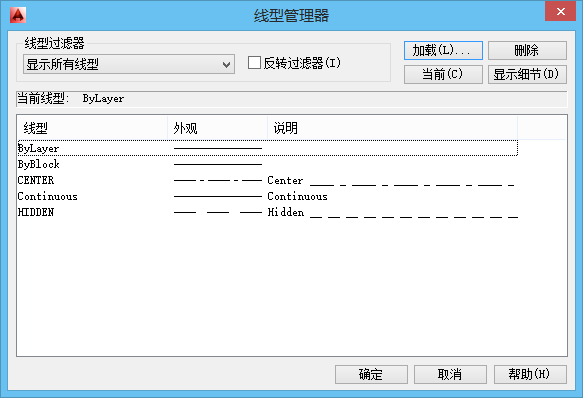
\includegraphics[scale=0.35]{loadhiddenline}}
\caption{线型管理}
\end{figure}

\begin{lstlisting}
命令: LINETYPE
\end{lstlisting}

\item 生成左视图

\begin{enumerate}
\item 新建左视图视口。

\begin{lstlisting}
命令: -VPORTS
指定视口的角点或 [开(ON)/关(OFF)/布满(F)/着色打印(S)/锁定(L)/对象(O)/多边形(P)/恢复(R)/图层(LA)/2/3/4] <布满>:
指定对角点:
\end{lstlisting}

\item 设置左视同图视口模型空间的视图方向为左视。
\begin{lstlisting}
命令: -VIEW
输入选项 [?/删除(D)/正交(O)/恢复(R)/保存(S)/设置(E)/窗口(W)]: left
\end{lstlisting}

\item 设置视口显示比例为1:1,结果如图\ref{fig:zhijiabuju3} 所示。

\end{enumerate}

\begin{figure}[htbp]
\centering
\begin{floatrow}[3]
\ffigbox[\FBwidth]{\caption{创建支架左视图显示}\label{fig:zhijiabuju3}}{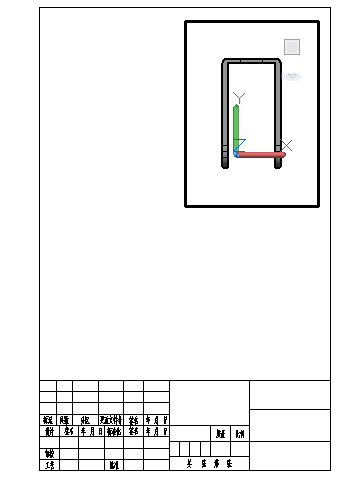
\includegraphics[scale=0.35]{zhijiabuju3}}
\ffigbox[\FBwidth]{\caption{创建支架主视图显示}\label{fig:zhijiabuju4}}{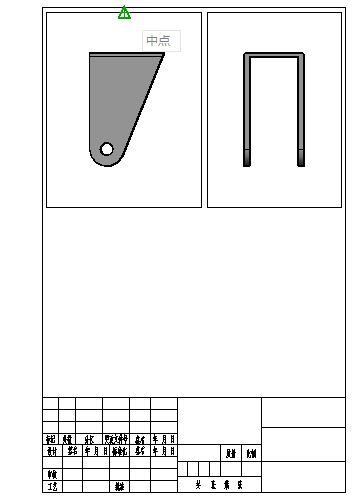
\includegraphics[scale=0.35]{zhijiabuju4}}
\ffigbox[\FBwidth]{\caption{创建支架俯视图显示}\label{fig:zhijiabuju5}}{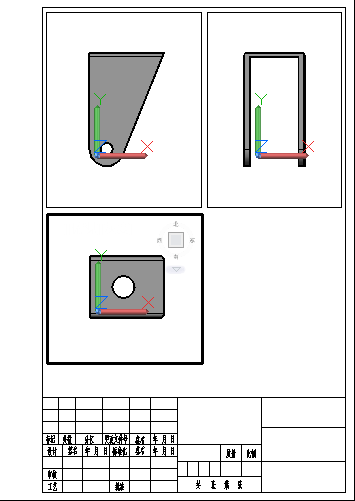
\includegraphics[scale=0.35]{zhijiabuju5}}
\end{floatrow}
\end{figure}

\item 生成全剖主视图

为更清楚地表达支架的内部结构,故采用全剖视图作为支架的主视图,能够实现既清楚表达支耳的结构又清楚表达顶板的孔。生成主视图的效果如图\ref{fig:zhijiabuju4}所示。

\begin{lstlisting}
命令: SOLVIEW
输入选项 [UCS(U)/正交(O)/辅助(A)/截面(S)]: s
指定剪切平面的第一个点:
指定剪切平面的第二个点:
指定要从哪侧查看:
输入视图比例 <1>:
指定视图中心:
指定视图中心 <指定视口>:
指定视口的第一个角点: 
指定视口的对角点:
输入视图名: front
输入选项 [UCS(U)/正交(O)/辅助(A)/截面(S)]:
\end{lstlisting}


\item 生成俯视图

双击进入主视图所在的视口模型空间,然后以主视图为基础用正交选项生成普通的俯视图,结果如图\ref{fig:zhijiabuju5}所示。

\begin{lstlisting}
命令: SOLVIEW
输入选项 [UCS(U)/正交(O)/辅助(A)/截面(S)]: o
指定视口要投影的那一侧:
指定视图中心:
指定视图中心 <指定视口>:
指定视口的第一个角点:
指定视口的对角点:
输入视图名: top
输入选项 [UCS(U)/正交(O)/辅助(A)/截面(S)]:
\end{lstlisting}

\item 生成左视图轮廓

到目前为止,还没有生成左视图。由于左视图是生成主视图的基础,因此只能用轮廓命令生成左视图。

\begin{lstlisting}
命令: SOLPROF
选择对象: 找到 1 个
选择对象:
是否在单独的图层中显示隐藏的轮廓线?[是(Y)/否(N)] <是>:
是否将轮廓线投影到平面?[是(Y)/否(N)] <是>:
是否删除相切的边? [是(Y)/否(N)] <是>:
\end{lstlisting}

\item 图形化主视图和俯视图

\begin{figure}[htbp]
\centering
\subfloat[]{\label{fig:zhijiabuju6}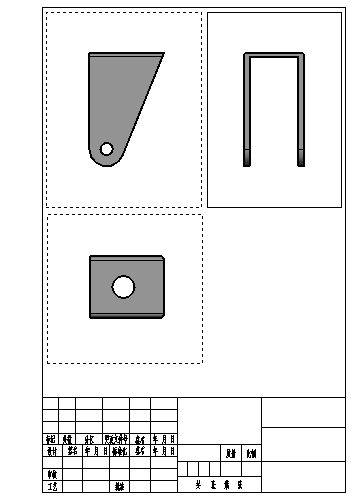
\includegraphics[scale=0.4]{zhijiabuju6}}\hspace{20pt}
\subfloat[]{\label{fig:zhijiabuju7}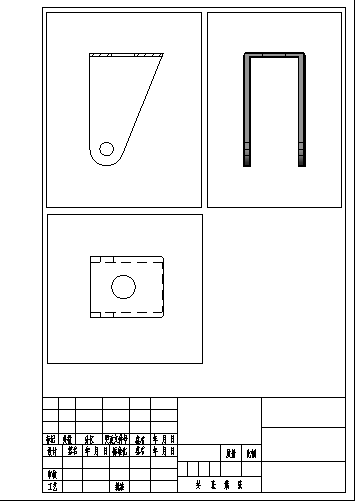
\includegraphics[scale=0.4]{zhijiabuju7}}
\caption{生成最终主俯视图}
\end{figure} 

选择主视图和俯视图作为图形化对象,选择后的效果如图\ref{fig:zhijiabuju6}所示。

\begin{lstlisting}
命令: SOLDRAW
选择要绘图的视口...
选择对象: 找到 1 个
选择对象: 找到 1 个,总计 2 个
选择对象:
\end{lstlisting}

\item 修改主视图图案填充

由于主视图的图案填充不符合国家标准的要求,故用图案填充编辑命令将填充图案修改为ANSI31。最终主视图和俯视图效果如图\ref{fig:zhijiabuju7}所示。

\begin{lstlisting}
命令: HATCHEDIT
选择图案填充对象:
\end{lstlisting}

\item 设置图层

按图\ref{fig:zhijiabuju8}进行支架的图层设置。
\begin{figure}[htbp]
\centering
\begin{floatrow}[2]
\ffigbox{\caption{支架图层设置}\label{fig:zhijiabuju8}}{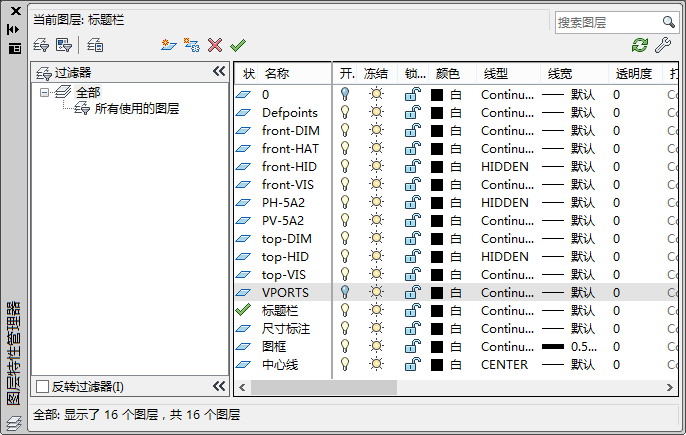
\includegraphics[scale=0.35]{zhijiabuju8}}
\ffigbox{\caption{绘制中心线结果}\label{fig:zhijiabuju9}}{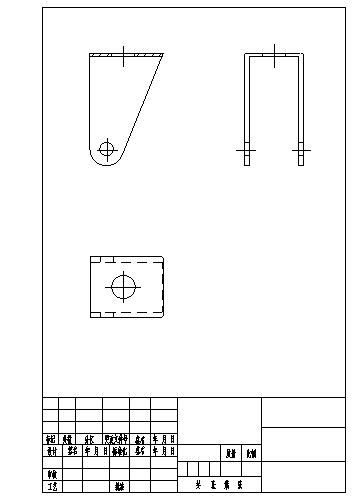
\includegraphics[scale=0.35]{zhijiabuju9}}
\end{floatrow}
\end{figure}
\item 绘制中心线

将当前图层设置为“中心线”图层,并绘制支架孔的中心线,结果如图\ref{fig:zhijiabuju9}所示。

\item 标注尺寸
\begin{enumerate}
\item 设置标注样式

按\ref{sec:lianjieganshitu}节的步骤设置标注样式。

\item 标注线性尺寸

完成支架三视图中所有线性尺寸的标注,结果如图\ref{fig:zhijiabuju10} 所示。

\begin{figure}[htbp]
\centering
\subfloat[]{\label{fig:zhijiabuju10}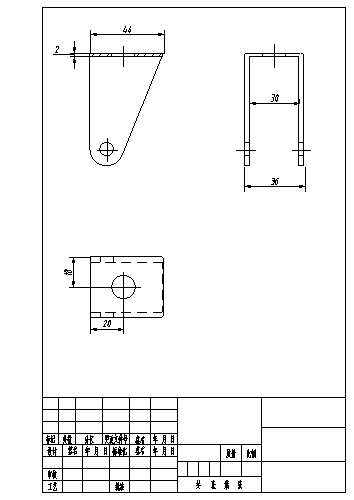
\includegraphics[scale=0.2]{zhijiabuju10}}\hspace{20pt}
\subfloat[]{\label{fig:zhijiabuju11}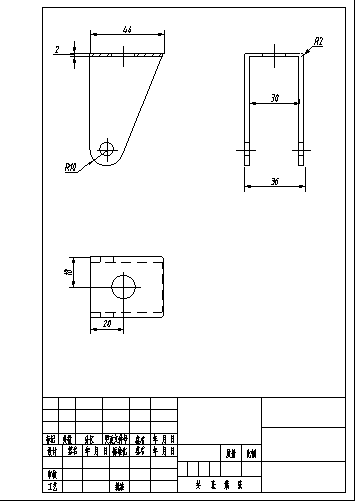
\includegraphics[scale=0.2]{zhijiabuju11}}\hspace{20pt}
\subfloat[]{\label{fig:zhijiabuju12}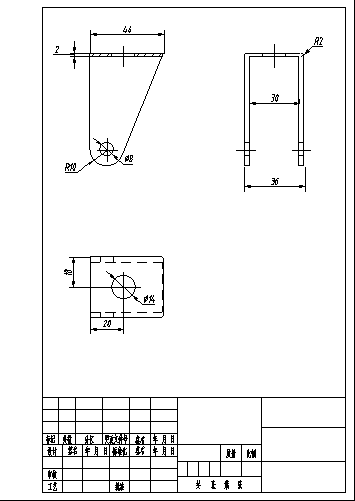
\includegraphics[scale=0.2]{zhijiabuju12}}\hspace{20pt}
\subfloat[]{\label{fig:zhijiabuju13}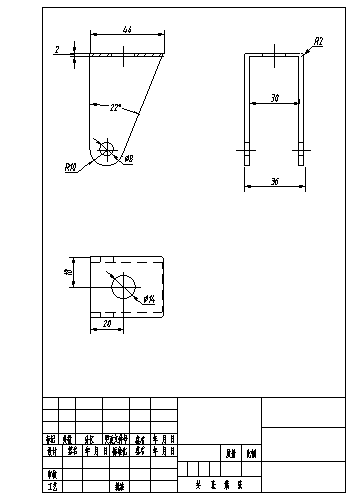
\includegraphics[scale=0.2]{zhijiabuju13}}
\caption{支架尺寸标注}
\end{figure}

\item 标注半径尺寸

完成支架三视图中所有圆弧的半径尺寸标注,结果如图\ref{fig:zhijiabuju11}所示。

\item 标注直径尺寸

完成支架三视图中所有圆的直径尺寸标注,结果如图\ref{fig:zhijiabuju12}所示。
\item 标注角度尺寸

对于支架中的角度尺寸需要调用AutoCAD中的角度标注命令,其方法有:
\begin{itemize}
\item 键盘输入dimangular\index{dimanglar,角度标注}
\item 【标注】$\rightarrow $【角度】
\item 【标注】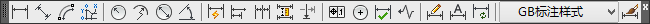
\includegraphics[scale=0.45]{dimtoolsbar}工具栏中的【角度】
\includegraphics[scale=0.45]{dimangular}图标
\end{itemize}

调用角度标注命令后,选择两条直线并指定标注线的位置即可完成角度标注,其结果如图\ref{fig:zhijiabuju13}所示。

\begin{lstlisting}
命令: dimangular
选择圆弧、圆、直线或 <指定顶点>:
选择第二条直线:
指定标注弧线位置或 [多行文字(M)/文字(T)/角度(A)/象限点(Q)]:
标注文字 = 22
\end{lstlisting}

\end{enumerate}

\end{procedure}
\endinput